%%%%%%%%%%%%%%%%%%%%%%%%%%%%%%%%%%%%%%%%%%%%%%%%%%%%%%%%%%%%%%%%%%%%%%%%%%%%%
%
%  System        : 
%  Module        : 
%  Object Name   : $RCSfile$
%  Revision      : $Revision$
%  Date          : $Date$
%  Author        : $Author$
%  Created By    : Robert Heller
%  Created       : Wed Nov 22 12:24:39 2023
%  Last Modified : <231122.1521>
%
%  Description 
%
%  Notes
%
%  History
% 
%%%%%%%%%%%%%%%%%%%%%%%%%%%%%%%%%%%%%%%%%%%%%%%%%%%%%%%%%%%%%%%%%%%%%%%%%%%%%
%
%    Copyright (C) 2023  Robert Heller D/B/A Deepwoods Software
%			51 Locke Hill Road
%			Wendell, MA 01379-9728
%
%    This program is free software; you can redistribute it and/or modify
%    it under the terms of the GNU General Public License as published by
%    the Free Software Foundation; either version 2 of the License, or
%    (at your option) any later version.
%
%    This program is distributed in the hope that it will be useful,
%    but WITHOUT ANY WARRANTY; without even the implied warranty of
%    MERCHANTABILITY or FITNESS FOR A PARTICULAR PURPOSE.  See the
%    GNU General Public License for more details.
%
%    You should have received a copy of the GNU General Public License
%    along with this program; if not, write to the Free Software
%    Foundation, Inc., 675 Mass Ave, Cambridge, MA 02139, USA.
%
% 
%
%%%%%%%%%%%%%%%%%%%%%%%%%%%%%%%%%%%%%%%%%%%%%%%%%%%%%%%%%%%%%%%%%%%%%%%%%%%%%

\documentclass[12pt,twoside]{article}
\usepackage{graphicx}
\usepackage{mathptm}
\usepackage{times}
\usepackage{makeidx}
\usepackage{ifpdf}
\ifpdf
\usepackage[pdftex,
            pagebackref=true,
            colorlinks=true,
            linkcolor=blue,
            unicode
           ]{hyperref}
\else
\usepackage[ps2pdf,
            pagebackref=true,
            colorlinks=true,
            linkcolor=blue,
            unicode
           ]{hyperref}
\usepackage{pspicture}
\fi
\usepackage{url}
\pagestyle{headings}
\makeindex
\emergencystretch=50pt
\setcounter{tocdepth}{3}
\setcounter{secnumdepth}{3}
\title{LCCCANCape: LCC CAN Tranceiver Cape (SMD version)}
\author{Robert Heller \\ The Country Robot \\ Wendell, MA, USA}
\date{\today}
\begin{document}
\maketitle

\section{GPIO Pins Used and stacking restrictions.}

This board uses two pins on header P9: 24 and 26 in pin mux mode2, which makes 
pin 24 Can1 RX, and pin 26 Can1 TX.  Only one of these capes can be on any 
Beagle Bone Black.


\section{Circuit Description}

\begin{figure}[hbpt]\begin{centering}%                                         
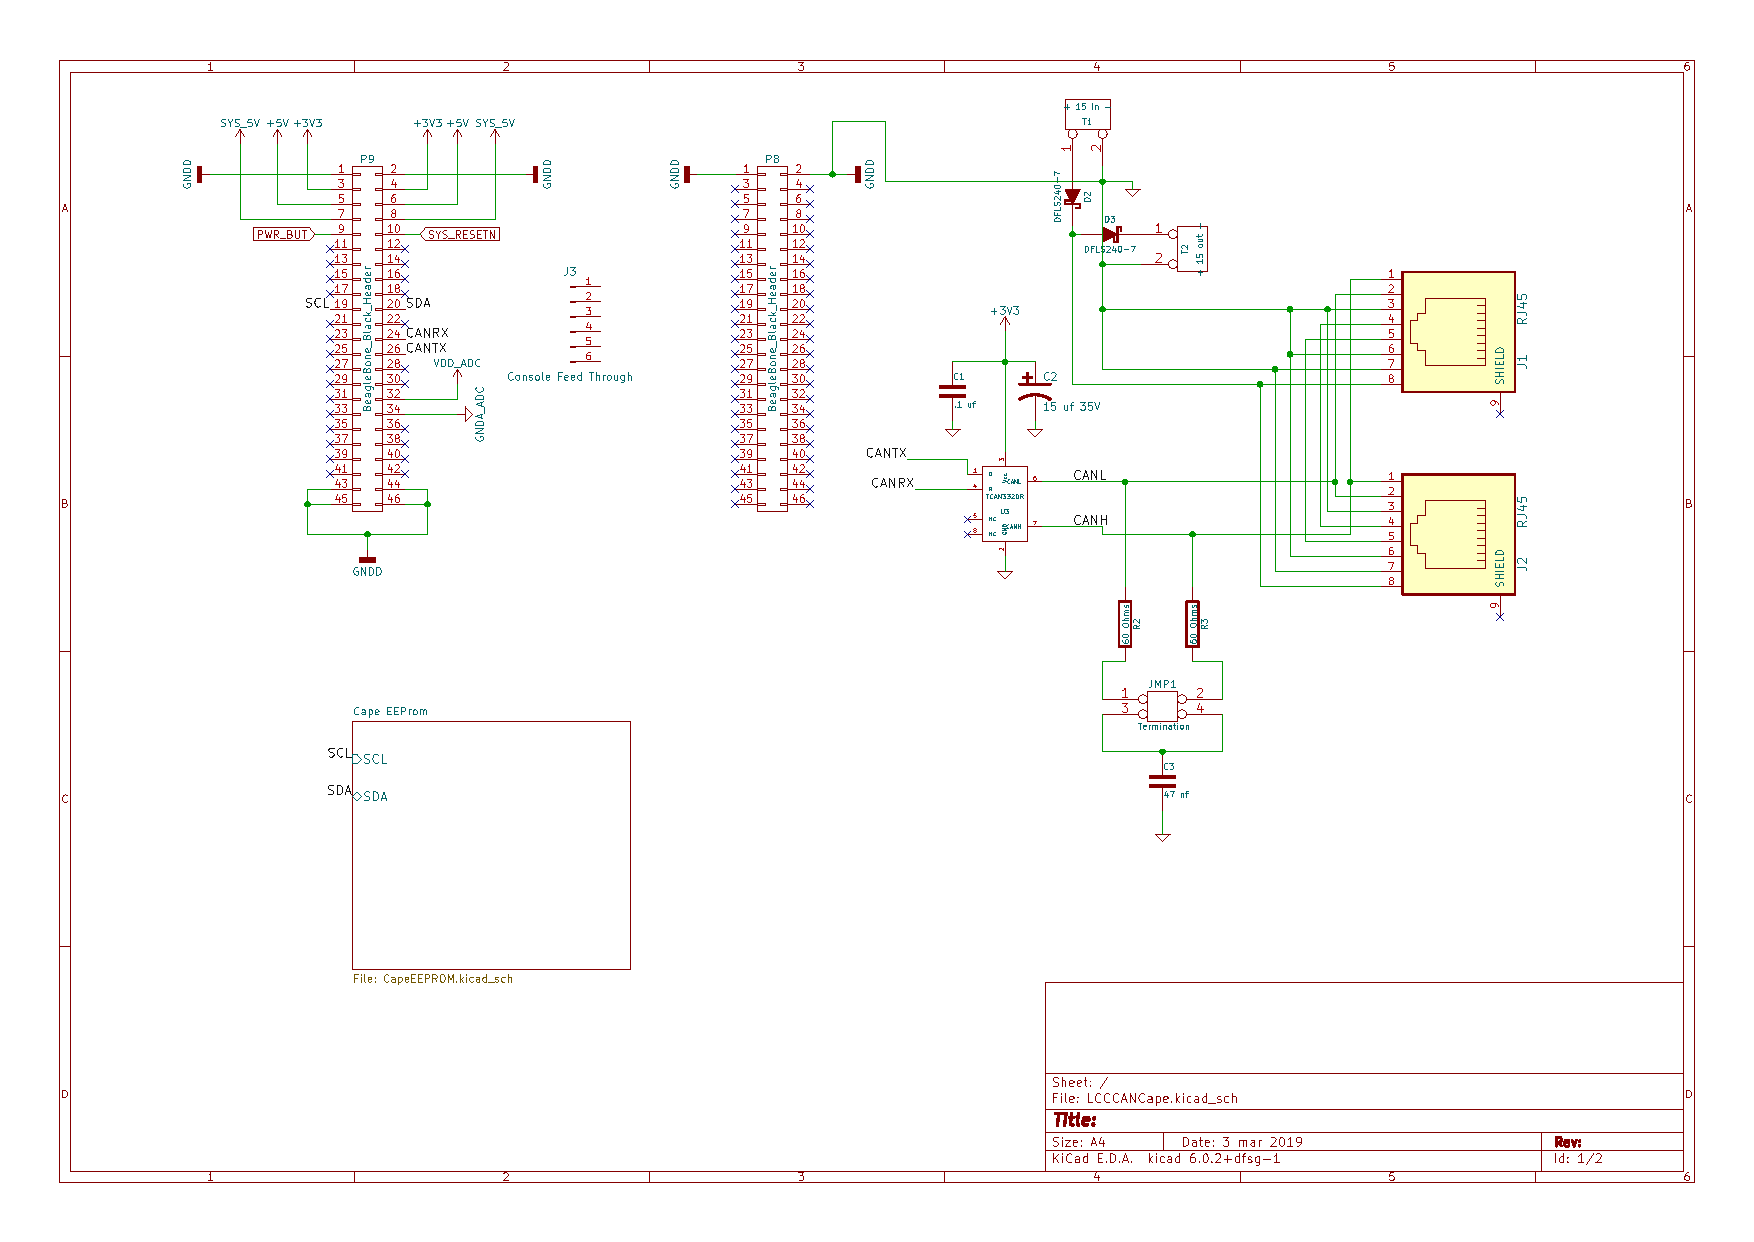
\includegraphics[width=5in]{LCCCANCape.pdf}                               
\caption{Circuit Diagram of the LCCCANCape}                               
\end{centering}\end{figure}                                                    
This circuit contains two sections.  There is the transciever section, which 
includes the transciver itself, the termination block, the two RJ45 jacks, and 
two terminal blocks for injecting and tapping into the power carried in the 
CAT 5 cable.  Power is not used to power the Beagle Bone Black.  The other 
section is the Cape EErom circuit.  The Cape EEProm contains         
information about the cape and the name and version of the overlay that needs  
to be loaded by uBoot.  

\clearpage

\section{Assembly Notes}
\begin{figure}[hbpt]\begin{centering}%
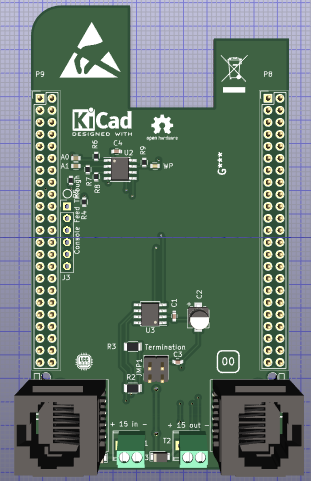
\includegraphics[height=5in]{LCCCANCape3DTop2.png}
\caption{3D top view of the LCCCANCape}
\end{centering}\end{figure} 

All of the parts are included. The Beagle Bone Header pins are mounted on the
bottom of the board (soldered on the top). You might want to replace the
Beagle Bone Header pins with stacking versions if you plan on stacking
additional capes (but note: the RJ45 connectors will interfere with standard
capes). 

\subsection{Solder bridges}
\label{sec:SolderBridges}

\begin{figure}[hbpt]\begin{centering}%
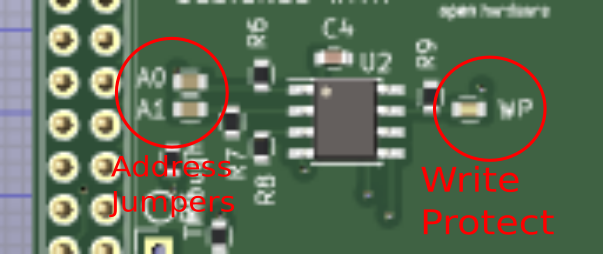
\includegraphics[width=4in]{LCCCANCape3DTop2_annotated.png}
\caption{Solder bridge locations}
\end{centering}\end{figure}

There are three solder bridges, two for addressing the ID PROM and one to
write protect the PROM.

\subsubsection{ID PROM addressing}

\begin{table}[htp]
\begin{centering}\begin{tabular}{|l|l|p{2in}|}
\hline
A0&A1&ROM/Cape Address\\
\hline
Bridged&Bridged&0x54 (Cape 0)\\
\hline
Unbridged&Bridged&0x55 (Cape 1)\\
\hline
Bridged&Unbridged&0x56 (Cape 2)\\
\hline
Unbridged&Unbridged&0x57 (Cape 3) This is the default.\\
\hline
\hline
\end{tabular}
\caption{ID PROM/Cape addressing.}
\end{centering}\end{table}

There are two solder bridges to addess the ID ROM/Cape. By default the bridges 
are open and thus the ID PROM is at 0x57 (Cape 3).

There is also a PROM Write protect jumper.  This jumper is bridged by default, 
which allows writing to the ID PROM.  Once you have written the ID content to 
the PROM, you can use a small knife to cut the trace shorting the jumper to 
write protect the PROM.

\subsection{ID PROM programming}

The ID PROM  should be programmed for proper operation.  The ID PROM is read 
during booting and will cause and device tree overlay to be loaded.  The device 
tree overlay will set things up to use the CAN interface.  Download the EEPROM 
binary from 
\url{https://www.thecountryrobot.com/wp-content/uploads/2023/11/LCCCANCAPE_CapeROM.zip} \\

\includegraphics[height=1in]{LCCCANCAPE_CapeROM_QR.png}.\\
This zip file contains the file \texttt{CapeROMSpec.bin}, which can be copyied 
to the EEPROM with these commands:

\begin{verbatim}
# Assumes the default address of 0x57.  If you have bridged the address 
# jumpers, change the address to match.
dd if=CapeROMSpec.bin of=/sys/bus/i2c/devices/2-0057/eeprom
dd if=/sys/bus/i2c/devices/2-0057/eeprom of=/tmp/eeprom.bin
diff -q CapeROMSpec.bin /tmp/eeprom.bin
\end{verbatim}

If there are no differences reported by diff, you can go ahead and cut the 
write protect jumper.

\section{Setting up the CAN socket device}

Add this text to \texttt{/etc/network/interfaces}:

\begin{verbatim}
auto can1
iface can1 inet manual
    pre-up /sbin/ip link set can1 type can bitrate 125000
    up /sbin/ifconfig can1 up
    down /sbin/ifconfig can1 down
\end{verbatim}

Then reboot the Beagle bone.

You should then see CAN1:

\begin{verbatim}
% ifconfig can1
can1: flags=193<UP,RUNNING,NOARP>  mtu 16
        unspec 00-00-00-00-00-00-00-00-00-00-00-00-00-00-00-00  txqueuelen 10  
(UNSPEC)
        RX packets 0  bytes 0 (0.0 B)
        RX errors 0  dropped 0  overruns 0  frame 0
        TX packets 0  bytes 0 (0.0 B)
        TX errors 0  dropped 0 overruns 0  carrier 0  collisions 0
        device interrupt 43  
\end{verbatim}

\section{Usage}

Any OpenMRN program (\url{https://github.com/bakerstu/openmrn}) natively built
on your Beagle bone can now use the LCC CAN IF on your Beagle bone. This
includes the hub program under applications -- this program can route LCC
traffic between the LCC CAN network and the Tcp/Ip network using the Beagle
bone's Ethernet. It is also possible to create your own OpenMRN node programs
using the Beagle bone's GPIO lines.

\end{document}

